\documentclass[11pt,a4paper]{article}
\usepackage[utf8]{inputenc}
\usepackage[T1]{fontenc}
\usepackage{amsmath,amssymb,bm}
\usepackage{geometry}
\usepackage{lmodern}
\usepackage{microtype}
\usepackage{hyperref}
\usepackage{tikz}
\usetikzlibrary{arrows.meta,decorations.markings}

\geometry{margin=2.5cm}

\title{Swirl--String Theory: Canon v0.4 \\ \large A Formal Axiomatic Framework}
\author{Omar Iskandarani\\\small Independent Researcher, Groningen, The Netherlands}
\date{September 2025}

\begin{document}
\maketitle

\section*{Abstract}
    We present Canon v0.4 of the Swirl--String Theory (SST), formally recast in Euclidean structure using axioms, definitions, lemmas, and theorems. Chirality and wave--particle duality emerge as consequences of the topology and dynamics of quantized circulation structures in a swirl field medium. We include structural diagrams and identify conjectural/empirical components separately in an appendix.

    \tableofcontents
    \newpage

\section{Axioms}

    \begin{axiom}[Swirl Flux Quantization]
    \label{ax:flux-quant}
    The total swirl flux through any closed 2-surface $A$ is quantized:
    \[
        \Phi_{\text{sw}} = \int_A \bm{\rho}_{\text{sw}} \cdot d\bm{A} = N\kappa, \quad N \in \mathbb{Z}.
    \]
    \end{axiom}

    \begin{axiom}[Chronos--Kelvin Invariant]
    \label{ax:chronos-kelvin}
    For any swirl flow on a time foliation leaf $\Sigma_t$, the following invariant holds:
    \[
        \frac{D}{Dt}(R^2\omega) = 0.
    \]
    \end{axiom}

    \begin{axiom}[Quantized Circulation]
    \label{ax:circulation}
    Each swirl loop carries quantized circulation:
    \[
        \Gamma_n = n\frac{h}{m_e}, \quad n \in \mathbb{Z}.
    \]
    \end{axiom}

\section{Definitions}

    \begin{definition}[Swirl Clock]
    \label{def:swirl-clock}
    The Swirl Clock $S_t^{\circlearrowleft}$ (or $S_t^{\circlearrowright}$) is the local time rate determined by swirl velocity orientation and magnitude, given by
    \[
        dt_{\text{local}} = dt_{\infty} \sqrt{1 - \frac{|\bm{v}_{\circlearrowleft}|^2}{c^2}}.
    \]
    \end{definition}

    \begin{definition}[Ring Phase $R$]
    The $R$ phase is a delocalized toroidal (unknotted) swirl-string with persistent circulation. It supports interference phenomena and corresponds to wave-like behavior.
    \end{definition}

    \begin{definition}[Knot Phase $T$]
    The $T$ phase is a localized, knotted string with positive curvature and topological helicity. It corresponds to particle-like, countable phenomena.
    \end{definition}

    \begin{definition}[Vortex Core Radius $r_c$]
    The minimal radial scale below which swirl structures collapse into discrete quantized cores.
    \end{definition}

\section{Lemmas and Theorems}

    \begin{lemma}[de Broglie Wavelength from Swirl Quantization]
    \label{lem:debroglie}
    For a ring phase of radius $R$, the wavelength is given by:
    \[
        \lambda = \frac{2\pi R}{n}, \quad \text{with } \Gamma_n = n\frac{h}{m_e}.
    \]
    \end{lemma}

    \begin{theorem}[R--T Transition by Photon Resonance]
    \label{thm:rt-transition}
    Let an $R$-phase swirl-string be exposed to a photon of energy $\hbar\omega$. The system transitions to a $T$-phase if:
    \[
        \hbar\omega \geq \Delta E_{\text{eff}}[K],
    \]
    where $K$ is the minimal knot state.
    \end{theorem}

    \begin{theorem}[Vortex Nucleation Threshold]
    \label{thm:nucleation}
    Given compressive swirl flux with spacing $a$, vortex lines must nucleate when:
    \[
        a \lesssim \alpha r_c,
    \]
    where $\alpha$ is a geometry-dependent constant.
    \end{theorem}

    \begin{corollary}[Fringe Visibility Decay]
    \label{cor:fringe}
    If $\Gamma$ is the knotting rate under EM interaction, interference visibility decays as:
    \[
        V(\Gamma, \tau) = e^{-\Gamma \tau}.
    \]
    \end{corollary}

\section{Illustrative Diagrams}

    \subsection*{Figure 1: Ring vs. Knot Phase Representation}
        \begin{center}
        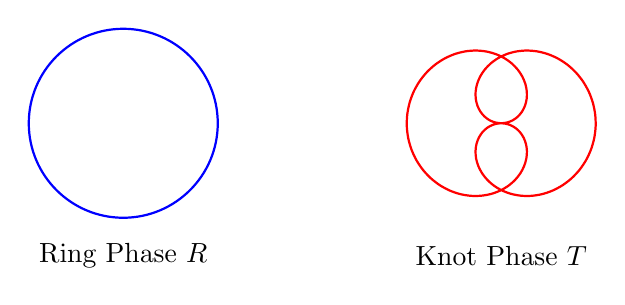
\begin{tikzpicture}[scale=1.2, thick]
% Ring
        \draw[blue, thick] (0,0) circle (1);
        \node at (0,-1.4) {Ring Phase $R$};

% Knot (simple trefoil shape)
        \begin{scope}[xshift=4cm]
        \draw[red, thick, domain=0:360, samples=100, smooth, variable=\t]
        plot ({sin(\t)*cos(2*\t)}, {sin(\t)*sin(2*\t)});
        \node at (0,-1.4) {Knot Phase $T$};
        \end{scope}
        \end{tikzpicture}
        \end{center}

    \subsection*{Figure 2: Swirl Flux Compression and Vortex Nucleation}
        \begin{center}
        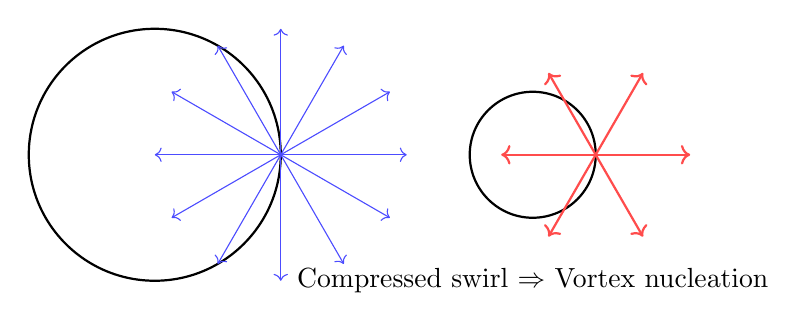
\begin{tikzpicture}[scale=0.8]
% Large circle with swirl lines
        \draw[thick] (0,0) circle (2);
        \foreach \angle in {0,30,...,330}
            {
            \draw[->, blue!70] (2,0) -- ++({\angle}:2);
        }

% Smaller compressed circle
        \begin{scope}[xshift=6cm]
        \draw[thick] (0,0) circle (1);
        \foreach \angle in {0,60,...,300}
            {
            \draw[->, red!70, thick] (1,0) -- ++({\angle}:1.5);
        }
        \node at (0,-2) {Compressed swirl $\Rightarrow$ Vortex nucleation};
        \end{scope}
        \end{tikzpicture}
        \end{center}

\section{Conjectures and Empirical Appendix}

    \begin{itemize}
    \item \textbf{Conjecture 1 (Dynamic Chirality):} Time-asymmetric photoionization delays result from Swirl Clock orientation.
    \item \textbf{Conjecture 2 (Topological Memory):} Knot phase $T$ retains initial swirl orientation beyond ionization.
    \item \textbf{Empirical Mapping:} Han et al. (2025) report $\Delta \tau = 60$–240 as; mapped via $\Delta \ell = v_e \cdot \Delta \tau$ to 0.5–4.5 \AA{} path differences.
    \end{itemize}

\end{document}